\section{Inledning}
\subsection{Teori \& bakgrund}
% Bakgrund

Automatiska växellådor sitter idag i en mängd av olika fordon,
däribland en helt elektrisk buss under utveckling av Volvo.
För att bland annat köra på rätt växel, optimera motorns styrprogram
och operera olika bromsfunktioner % och vad mer/något mer?
mätes fordonets lutning.
För det ändamålet ska lutningsgivare användas.
Lutningsgivaren är en fristående modul som kommunicerar med styrdatorn via
Controller Area Network (CAN)-kommunikation.
Detta fungerar bra vid rörelse i konstant hastighet
men vid accelereration uppstår mätbrus och andra störningar.
Därför behövs en algoritm för att felkompensera dessa störningar.

%teori
% - piezoelekrtiskakristaller
% - algoritmen

Piezoelektriska material, har en kristallstruktur och, ger upphov till
elektriska laddningar på dess yta under yttre mekaniskt tryck, den så kallade
direkta piezoelektriska effekten.
Det mekaniska arbete som utförs omvandlas till elektricitet, det omvända gäller
också, elektricitet omvandlas till mekansikt arbete i den omvända
piezoelektriska effekten i vilken kristallen deformeras.
\autocite{electronicdesign2016}
Piezoelektriska lutningsgivare använder elektriska signaler som är
inducerade via den piezoelektriska effekten från en piezoelektrisk kropp
under gravitationskraften från en tyngd.
Vinkeln mellan gravitationskraften och
riktningen på den piezoelektriska kroppens vibration
fås av att man mäter magnituden av kraftenkomponenten i vibrationens riktning
och använder geometriska samband mellan dem.
\autocite{chiang00}

%vad neuronnät är och vad de används till
Ett artificiellt neuronnät är ett en självlärande algoritm som inspirerats av
hur djurs hjärnor fungerar och kommunicerar.
Neuronnät kan användas för att klara av vissa problem som annars är svårlösta
med konventionella datalogiska metoder.
Ett neuronnät ``lär sig'', precis som vi gör, genom att observera.
Men för att ha avsedd funktion måste de tränas, alltså är arbete med neuronnät
uppdelat i två faser: en inlärningsfas och en tillämpningsfas där nätverket sedan
utför den ämnade uppgiften.
\autocite{copeland16}

%sigmoid neuroner
%TODO bli konsekvent i hur begrepp ska skrivas, alltså språk osv.
Ett neuronnät består av sigmoidneuroner %hur ska sigmoid neuronerna stavas
för att en liten förändring i en \textit{weight} eller \textit{bias}) ska resultera
i en liten förändring i ``utmatningen'' (från eng. \textit{output}).
För då är det möjligt att gradvis ``träna'' nätverket till att %...
Inmatningen (från eng. \textit{input}) till en sigmoidneuron är alltså ett
tal mellan 0 och 1.
\autocite{nielsen15}

% Förlustfunktionen
Med hjälp av en slät funktion för hur väl nätet approximerar träningsdatan
kan man korrelera små ändringar i weights och biases
till små förbättringar i prestandan.
Den \emph{kvadratiska förlustfunktionen} är en sådan funktion:

\begin{equation}
	C(w, b) \equiv \frac{1}{2n} \displaystyle\sum_x \lVert y(x) - a \rVert^2
\end{equation}

där $ w $ är alla weights i nätet, $ b $ är alla biases,
$ n $ är antalet träningsindata, $ a $ är en vektor med utdata när $ x $ är indata
och summan är över all träningsindata $ x $.
Man ser att $ C(w, b) $ är icke-negativ då varje term i summan är positiv.
Dessutom är förlusten $ C(w, b) $ liten, det vill säga $ C(w, b) \approx 0 $,
när $ y(x) $ är ungefär lika med utdatan, $ a $, för alla träningsindata, $ x $.
Målet med träningsalgoritmen blir då att minimera $ C(w, b) $.

\begin{figure}
	\centering
	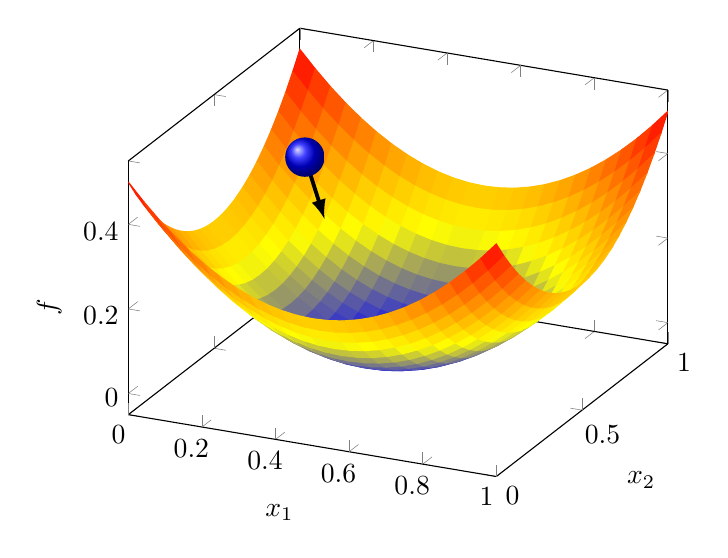
\begin{tikzpicture}
		\begin{axis}[domain=0:1,xlabel={$x_1$},ylabel={$x_2$},zlabel={$f$}]
			\addplot3[surf,shader=flat] {(x-0.5)^2 + (y-0.5)^2};
			\draw[->,line width=0.004\linewidth,>=latex] (axis cs:0.2,0.6,0.4) -- (axis cs:0.3,0.5,0.3);
			\node[circle,shading=ball,minimum width=0.5cm] (ball) at (axis cs:0.2,0.6,0.4) {};
		\end{axis}
	\end{tikzpicture}
	\caption{Gradient descent}
	\label{fig:descent}
\end{figure}

En algoritm för det är \emph{gradient descent}.
Om man föreställer sig en funktion $ f(x_1, x_2) $ som en dal,
se figur~\ref{fig:descent},
säger intuition att en boll skulle rulla ner för sluttningen till botten.
Vi kan simulera detta genom att räkna ut gradienten av $ f $.
Gradienten av $ f $, $ \nabla f $, vid en punkt är en vektor
som pekar i riktningen av den brantaste lutningen vid den punkten:

\begin{equation}
	\nabla f = \begin{bmatrix} \frac{\partial f}{\partial x_1} & \frac{\partial f}{\partial x_2} \end{bmatrix}^{T}
\end{equation}

där $ \partial f / \partial x_i $ är den partiella derivatan
som beskriver hur snabbt $ f $ växer med avseende på variablen $ x_i $.
Vi kan minska $ f $ genom att gå i riktningen av den negativa gradienten:

\begin{equation}
	x \rightarrow x' = x - \eta \nabla f(x)
\end{equation}

där $ \eta $ är inlärningshastigheten,
en positiv skalär som bestämmer längden av steget.

\subsection{Syfte}
Syftet med undersökningen är att ta fram och utvärdera en algoritm med
artificiella neuronnät som felkompenserar lutningsgivare i elbussväxellådor.

\subsection{Frågeställningar}
Vi vill undersöka\ldots
\begin{itemize}
	\item Varför råsignalen från lutningsgivaren blir opålitlig.
	\item Hur nätverket ska vara konfigurerat för att felkompensera; vilka inputs,
		outputs, antal neuroner, hidden layers och feed-/cascade-forward?
	\item Hur väl det fungerar att felkompensera med neuronnät.
\end{itemize}
